\startchapter{Phase sensitive radar reveals year long consistent basal layer of marine ice at apex of basal channel}
\label{ch:apres}



\section{Introduction --- section headings will be removed}



\subsection{Justification}

Ice shelves are a control on Antarctica's mass balance, providing resisting stresses  which slow ice discharge at the outlets of glaciers and ice streams  \citep{de2003glacier,gudmundsson2003transmission,dupont2005assessment}.
Melt at the base of ice shelves accounts for roughly half of ice shelf mass loss in Antarctica \citep{rignot2013ice}. To constrain and improve the accuracy of  forecasts of the mass balance and buttressing ability of ice shelves it is necessary to quantify modern basal melt  \citep[e.g.][] {furst2016safety}. 

% Floating ice shelves around Antarctica are thinning substantially, driven primarily by melting at the ice-ocean interface [Paolo et al., 2015; Rignot et al., 2013]. On a regional scale this thinning is well mapped, but small-scale local melt patterns are not well known. Uneven melt distribution leading to channel formation may significantly influence the total mass loss of ice shelves and alter their buttressing ability, surface velocity, and basal basal mass balance

\begin{figure}[!ht]
\centering
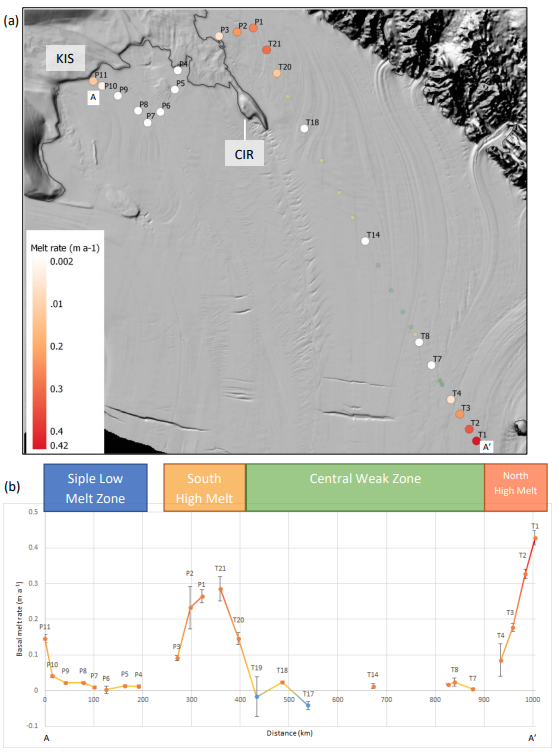
\includegraphics[width=0.5\textwidth]{chapters/3/RIS_melt.png}
\caption[]{From \cite{snodgrass2021melting}. Basal basal mass balance across the Ross Ice Shelf in (a) map view (b) and by distance along
the transect. Error bars indicate ApRES error. Yellow and green
markers on the map view indicate site locations where melting could not be quantified.  }
\label{fig:RIS_melt}
\end{figure}  

%\subsection{(temp) Ice shelf melt overview}

At a large scale, basal ice shelf melt is driven by the circulation of water from the open ocean. This circulation is described in detail by \cite{jacobs1992melting} and summarised here. The freezing of sea ice on the open ocean forms dense high salinity water which flows along the bottom of the ice shelf cavity to the grounding line. When this relatively warm, salty layer contacts grounded ice, it melts the ice base and forms melt--water plumes. The fresh plumes, driven by buoyancy, flow seaward along the upward sloping ice shelf base at the ice--ocean interface. As the buoyant plumes continue to rise they decrease in pressure, becoming super cooled, and partially freezing to the ice base \citep{lewis1986ice}.  
Due to this circulation pattern, melting is greatest at the perimeter of an ice shelf: at the ice front where ice is in close contact with open ocean \citep[e.g.][] {goldberg2019accurately}, and the grounding line \citep[e.g.][] {mankoff2012role}, where deeper ice is in contact with warm salty water which sits at the bottom of ice shelf cavity. In the centre of an ice shelf, the ice--ocean interface is generally at equilibrium or shows accretion \citep[e.g.][] {rignot2013ice}. This pattern is clear in the basal mass balance recorded by a traverse of the Ross Ice Shelf by \cite{snodgrass2021melting} shown in Figure \ref{fig:RIS_melt}.

\subsection{Observations of ice shelf melt}
While these theories of ocean circulation are generally supported by direct observations, such generalisations neglect small scale variations in basal mass balance which are commonly observed, both temporally \citep[e.g.][]{stewart2018ice} and spatially \citep[e.g.][]{marsh2016high}.

%\subsubsection{(temp) Observations of temporarily changing melt}

Temporal changes in basal melt can be observed directly using acoustic altimeters \citep[e.g.][]{stewart2018ice}. Basal accretion is often observed directly, though can be challenging to quantify \citep{vavnkova2020observations}. In supercooled water oceanographic instruments interfere with accretion, and accretion of ice to sensors disrupts measurements \citep{robinson2020ice}.   In the centre of the Ross Ice Shelf, \cite{stevens2020ocean} observed a 10 cm layer of ice crystals during melt conditions, which they interpreted as displaying the ablation phase of intermittent melt and accretion.  Similarly, \cite{craven2014platelet} interpreted the floating and sinking of moored instruments as intermittent accretion and melting.

Alternatively, the surface--based Autonomous Phase-sensitive Radio-Echo Sounder (ApRES) instrument surveys precise measurements of melt rates on ice shelves by comparing small changes in the phase of radar waves reflected off the ice base between repeat radar surveys. 
Relative to drilling a hole through the ice shelf to access the basal interface directly, ApRES surveys are inexpensive in resources and time. ApRES can be used to better understand processes in ice \citep[e.g.][]{case2022phase} and at the ice base \citep[e.g.][]{sun2019topographic}.  However, inference of basal processes with ApRES is an estimation which relies on assumptions about the properties of the ice and ocean outlined in Section \ref{sec:method} \cite{brennan2014phase}.
The ApRES was primarily designed for observing negative basal mass balance (melt). Most ApRES surveys observe basal melt, \citep[e.g.][] {lindback2019spatial,davis2018variability}, however, the ApRES has been used to observe accretion \citep[e.g.][] {stewart2018ice}, and new techniques are being developed to improve the interpretation of accretion \citep{vavnkova2020observations}. 

% Some new methods are being developed to improve processing of accretion time series for example . 

ApRES time series of basal melt under ice shelves can reveal connections between certain ocean forcings and the ice--ocean interface. While melt time series close to the front of ice shelves generally show seasonality and relationships with ocean conditions \citep[e.g.][]{lindback2019spatial}, time series from further inland are often difficult to interpret and show little connection to our understanding of ocean circulation \citep[e.g.][]{davis2018variability}. 
\cite{lindback2019spatial} present two ApRES time series of basal melt from the Nivlisen ice shelf. The first, 4 km from the ice front, shows seasonality while the second, 35 km from the ice shelf front, does not. Both sites show diurnal periods, semidiurnal periods and a fortnightly period, which the authors attribute to tidal cycles. 
 %see lindback for fourier analysis
Similarly, \citet{sun2019topographic} record basal melt about 90 km from the ice shelf front, near the grounding line of the Roi Baudouin Ice Shelf and see no seasonality though find a diurnal period which they attribute to a tidal cycle. 
Alternatively, \cite{hirano2020strong} see strong seasonality in basal melt at a location 45 km inland from the of the Shirase Glacier Tongue, 16 km from the north of the southernmost SGT grounding line.
At a location hundreds of kilometres from the open ocean, \citet{vavnkova2020observations} observe little periodicity though see intermittent melt and accretion. 


%\subsubsection{(temp) Observations of spatially changing melt}
% While studies have quantified melt fairly accurately over large spatial scales ($>$1km) with remote sensing techniques \citep[e.g.][] {mankoff2012role}, ground based surveys have revealed that melt varies over smaller spatial scales ($\approx$ 100 m), particularly at channels in the ice base. Such channels may redistribute melt by affecting ocean circulation \citep[e.g.][] {goldberg2019accurately}, and change the structural rigidity of ice shelves \citep[e.g.][]{alley2019troughs}.

Typically, direct observations of the ice base are restricted to point surveys. Because drilling through an ice shelf is resource intensive, these measurements are sparse.  Submarine technology opens up possibilities for spatial surveys of the ice base, but have not yet been used to survey ice base mass balance.
As a result, most spatial surveys of basal mass balance come from indirect remote sensing techniques and ApRES.  

At a coarse resolution ($>$1km), basal mass balance has been mapped over large areas of Antarctica's ice shelves using remote sensing techniques \citep[e.g.][] {rignot2013ice, mankoff2012role,goldberg2019accurately}. Using velocity data to estimate flux divergence, mass conservation is solved for the basal mass balance. A detailed description of these techniques can be found in \cite{berger2017detecting}.
Over large scales these studies have confirmed that melting is greatest at the perimeter of an ice shelf: at the ice front where ice is in close contact with open ocean and the grounding line \citep[e.g.][] {rignot2013ice, mankoff2012role,goldberg2019accurately}, and at the grounding line where deeper ice is in contact with warm salty water at the bottom of ice shelf cavity. 
However these techniques rely on the assumption that ice is at hydrostatic equilibrium, so  begin to fail at a length scale where ice is not at equilibrium. This occurs at lengths approximately greater than ice thickness \citep{gudmundsson2008limit},  ($\gtrapprox$ 100s of m for ice shelves).

To resolve basal mass balance at higher spatial resolution it is common to use ground based ApRES, whereby point locations are surveyed twice at different times, and basal mass balance is calculated from the change in radar reflection \citep{stanton2013channelized, dutrieux2014basal,marsh2016high}. Such surveys have revealed large changes in basal mass balance over scales of hundreds of metres. These high gradients in basal melt have been found at the ice front \cite[e.g.][]{stewart2019basal} and at basal channels \citep[e.g.][]{stanton2013channelized, marsh2016high}. 
For example, \cite {marsh2016high} and \cite{stanton2013channelized} used ApRES to measured melt rates of 22.2 $\pm$ 0.2 m/yr and 14.2 to 24.5 m/yr in channels on the ice shelves of the Whillans Ice Stream and Pine Island Glacier respectively. In both cases, melt rates were measured near-zero outside of the channel, 1-2km and 200 m away from the channel apex respectively.

% The spatial resolution of  measurements depends on the topography of the basal reflection. On a perfectly flat based ice shelf, radar does theoretically have limits on spatial resolution. However, large features, such as a basal crevass or channel may cause off nadir reflections which may obscure nearby parts of the base \citep{vavnkova2021deriving}. When imaging just nearby a large reflector, the high amplitude primary return from the reflector dominates the signal and the later reflection of the bed may be difficult to distinguish.
% Higher resolution surveys of basal mass balance, have revealed large changes in basal mass balance over small scales. For example, \cite{chartrand2020basal} estimated basal mass balance at the apex of a basal channel to be 22 m/yr while 2-3 km away basal mass balance decayed to zero.  Channels are observed on ice sheets across Antarctica, and are thought to concentration  buoyant meltwater plumes. See Chapter \ref{ch:data} for a more detailed description of channel formation.  have been used to observe changes in basal mass balance at channels  
% Because ApRES can be used to observe the ice base from  the surface, it is a popular method to carry out spatial surveys of basal mass balance \citep{stanton2013channelized, marsh2016high}.

\subsection{Goal and Structure}
Here we present a time series of ApRES observations in a location situated at the apex of a basal channel at the grounding line of the Kamb Ice Stream (Figure~\ref{fig:geophysics_overview_apres}).  The objective of this chapter is to constrain processes at, and structure of the ice--ocean interface. We aim to identify changes (or lack of changes) in basal mass balance, and associate those changes to large processes in the channel, e.g. tides or subglacial drainage.
 The channel has been identified in previous studies by \cite{alley2016impacts,kim2016active,goeller2015subglacial} and \cite{horgan2017poststagnation}. These authors proposed that the channel is sourced by subglacial drainage from the main trunk of the Kamb Ice Stream. A cross section of basal mass balance bisecting the channel was presented in Chapter \ref{ch:data}.

In this chapter, we start by describing data processing  which follow the method of \cite{nicholls2015ground}, using code from \cite{stewart2018ice} and accretion methods from \cite{vavnkova2021nature} (Section \ref{sec:method}). In Section \ref{sec:method} we refer to the basal mass balance observed with the ApRES as `melt rate' in line with ApRES nomenclature. In Section \ref{sec:results}, results from the time series are presented, including time series of apparent accretion rates, the amplitudes of the basal reflector, and strain rates. In this section, we use the terminology coined by \cite{vavnkova2021nature}, referring to the observed basal mass balance as `apparent accretion'. Apparent accretion refers to the change in basal mass balance estimated using a dielectric constant of glacial ice to convert phase to displacement, substituting the unknown electromagnetic properties of the accreted marine ice (as described in Section \ref{sec:method}), and neglecting the effects of multiple basal reflections.
 Lastly, we discuss the physical meaning of apparent accretion rate, and implications of the time series (Section \ref{sec:discussion}).

\subsection{Site description}
\newpage
\begin{figure}[!ht]
\centering
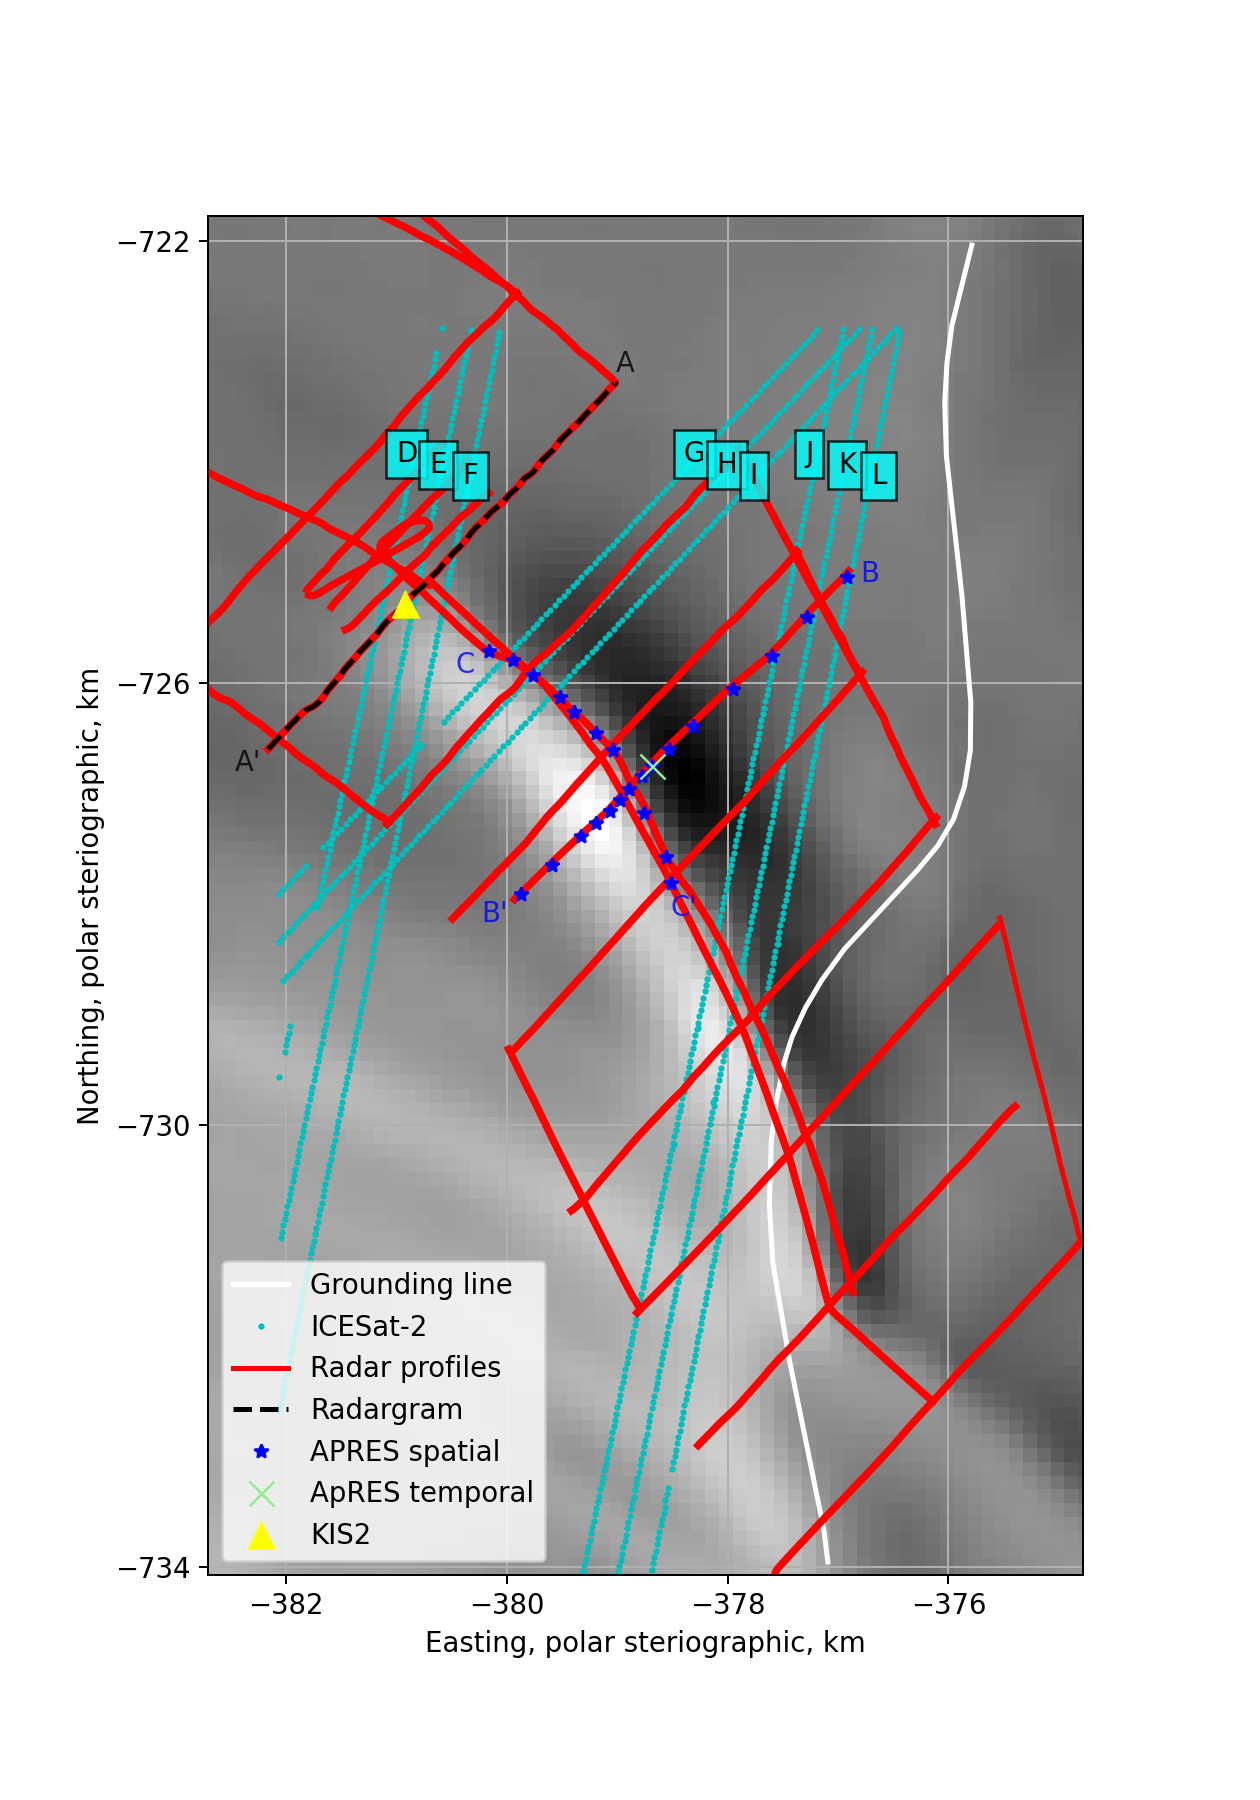
\includegraphics[width=0.6\textwidth]{chapters/2/geophysics_overview.png}
\caption[]{Map of study area showing all field data. Ice flow direction is from top left to bottom right. Background image is MODIS MOA 2009 \citep{haran2014modis}. Red lines are low--frequency radar profiles, white line is grounding line from \cite{depoorter2013amii}, black dashed line shows location of radar profile from Figure S6, blue dots are ApRES measurement locations, and light blue dots are ICESat--2 tracks.  ApRES was placed continuously recording at the light green `X', and the yellow triangle marks the planned location of a direct access drilling site scheduled for drilling in late 2021. Letters are labels referred to in subsequent figures.}
\label{fig:geophysics_overview_apres}
\end{figure}


To estimate basal mass balance at a channel incised into the base of the Ross Ice Shelf, an Autonomous Phase-sensitive Radio-Echo Sounder (ApRES) was deployed. The channel extends upstream of the grounding line of the Kamb Ice Stream. 
The site location (Figure \ref{fig:geophysics_overview_apres}) is at the apex of a basal channel, where ice thickness is 433 metres. 
The channel is manifest on the ice surface as a 10,000 x 3000 x 20 m valley, and is clearly visible from the ground and in satellite imagery. 
The ApRES instrument was 3 km from the inception of the channel and 3 km upstream from the Ross Ice Shelf cavity. The instrument was installed on 31st of December 2019, and retrieved on the 24 December 2020. 
Radar imagery described in Chapter \ref{ch:data} shows that the basal channel extends 6 km upstream of the previously estimated grounding line of the Kamb Ice Stream and incises up to 50\% of the ice thickness.  Because the channel is situated at the outlet of estimated subglacial drainage paths (Chapter \ref{ch:data}), the channel is likely formed by a buoyant meltwater plume triggered by subglacial discharge \citep{kim2016active}. 
Remote sensing data shows present day surface lowering at the head of the channel, which in Chapter \ref{ch:data} we interpret as submarine melt. 


\section{Methods} \label{sec:method}

\subsection{Field}
\begin{figure}[!ht]
\centering
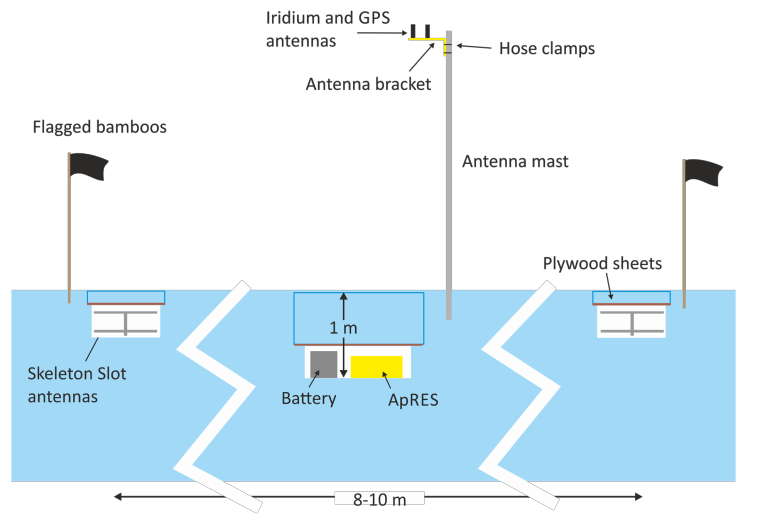
\includegraphics[width=0.8\textwidth]{chapters/3/apres_setup.png}
\caption[]{Image from \cite{nicholls2018apres}, ApRES setup with two skeleton slot antennas, a gps on a mast to keep the internal clock synchronised, a battery, and a box labelled `ApRES' with radar board and radar controller enclosed.}
\label{fig:apres_setup}
\end{figure}

Developed by \cite{brennan2014phase} and \cite{nicholls2015ground}, ApRES uses multiple frequency radio waves to image the ice base and internal ice reflectors to detect high spatial resolution mass balance.
ApRES is a frequency modulated continuous wave system, which unlike single frequency radar, generates and emits a continuous wave signal. The system's advantage over traditional radar systems is a superior signal to noise ratio. The instrument (Figure \ref{fig:apres_setup}) consists of two skeleton slot antennas, a GPS to keep the internal clock syncronised, a battery, and an enclosed radar board and radar controller, which also logs the data. The ApRES was deployed following \cite{nicholls2018apres}, with antenna $\approx 9$ m apart, 1 m deep and with parallel orientation. The instrument set up is shown in Figure \ref{fig:apres_setup}. 

The ApRES was set up to survey the ice every hour through the following procedure:
The first antenna transmitted a sequence of 20 chirps of radio waves. Each chirp ramped linearly from 200 to 400 MHz over a 1s period. The second antenna received the signal,  first passing it through amplifiers, and an adjustable attenuator set on deployment.  %craig thesis
The received signal and a copy of the transmitted signal was then multiplied with a frequency mixer, in a process known as deramping. This removed the linear ramp of frequencies produced by a chirp, and produced an output signal with frequencies of the sum and differences of the received and transmitted signal. This was low pass filtered to isolate the difference,  which contains a beat frequency proportional to the range, or distance from the antenna to the basal reflector. 
The signal was then high--pass filtered, amplifying weaker, more distant reflections to correct for effects of geometric spreading and dielectric absorption.  



%https://www.researchgate.net/publication/280912541_Effects_of_radar_side-lobes_on_snow_depth_retrievals_from_Operation_IceBridge

\subsection{Processing}

Data processing followed \cite{brennan2014phase} and \cite{nicholls2015ground}. The methods described by these authors is summarised here.

The frequency of the deramped signal, $f_d$ is given by
\begin{align}
    f_d = \frac{2 B \sqrt{\epsilon_r}}{Tc},
\end{align}
where $T$ is the pulse duration, $c$ is the speed of light, $B$ is the sweep bandwith and $\epsilon_r$ is the dielectric constant of the medium (genrally $3.1$ for ice).
The range to a reflection is an average across the radar footprint. The range resolution, $\Delta R$, is the minimum vertical distance at which two separate reflections can be resolved.
$f_d$ is found using Discrete Fourier Transform of the deramped signal, resulting in a spectral estimate with a resolution of $\Delta f_d = 1 /T$. This implies a range resolution between Discrete Fourier Transform bins of
\begin{align}
    \Delta R = \frac{c}{2B \sqrt{\epsilon_r} },
\end{align}
and a range to the nth Discret Fourier Transform bin centre of
\begin{align}
    R_{coarse}(n) = \frac{n c}{2B},
\end{align}

valid only for bins from $n = 0$ to $n= N/2 -1$.%where N is the number of samples in the digitised signal.
A typical centre frequency of 300 MHz and a sweep bandwidth of 200 MHz correspond to a deramped frequency of 2.35 Hz/m, with 1 s pulses. This gives a range resolution of 43 cm \cite{brennan2014phase}.
The phase of the deramped signal is also proportional to target range. The phase range estimate can be combined with the frequency-derived range to obtain absolute range measurements with sub-mm precision \cite{brennan2014phase}. To maintain accurate phase-coherency between signals, the exact time at which the signal is digitised is aligned with the start of each transmitted chirp. The fine range,
\begin{align}
    R_{fine} = \frac{\lambda \phi_d}{4 \pi}
\end{align}
was used to find the difference in phase between a Discrete Fourier Transform bin centre and the reflector \cite{brennan2014phase}, where $\lambda$ is the wavelength in the medium and $\phi_d$ is the is the instantaneous phase of the deramped signal at the chirp centre.
When combined with the coarse range, total range can be resolved at millimetre accuracy. 
ApRES was primarily designed to measure melt at the base of ice shelves. For a melt application, it is assumed that a temporal phase shift is caused by a vertical displacement of the basal reflector. This neglects phase changes in the dieletric contrast of the reflector caused by changes in ice or ocean properties at the reflector interface, which are small under melt conditions. Under  conditions like at the Ross Ice Shelf, where the salinity is $\approx$ 34 psu, even a relatively large change of 4 psu would result in an apparent thickness change of less than 0.1 mm.
Under conditions of basal accretion changes in the electromagnetic properties of accreted ice affect the phase of the reflection. In this case, it is no longer appropriate to interpret changes in phase solely as changes in ice thickness.


\begin{figure}[!ht]
\centering
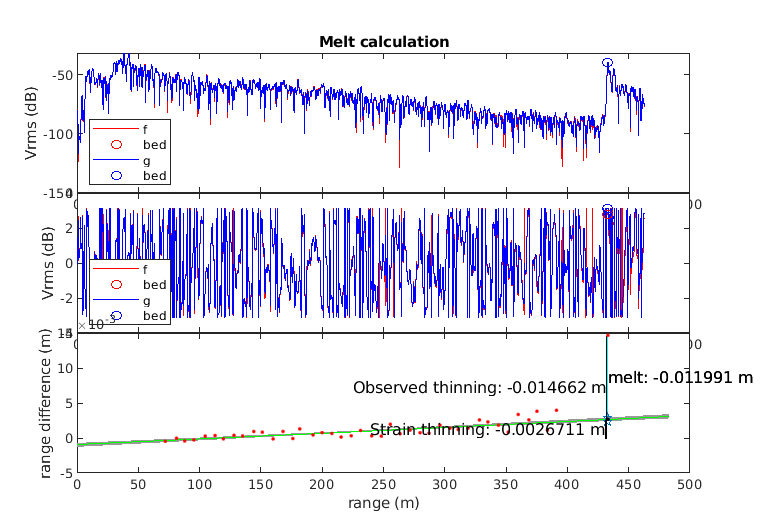
\includegraphics[width=1\textwidth]{chapters/3/melt_calc.png}
\caption[]{Example signals from repeat ApRES radar surveys 140 hours apart. A) The fourier transform of the averaged radar chirp, amplitude of the return signal as a function of depth. The clear basal reflection is at 433 m. B) The radar signal
C) Vertical displacement of tracked internal reflectors (red dots). The green line shows the linear fit through internal reflectors, and the red stars show the observed displacement of the shelf base, and the displacement due to vertical strain. The black vertical line shows the distance between extrapolated strain and the basal reflector, representing estimated melt. Blue stars show the bounds of estimated strain error. }
\label{fig:example_signal}
\end{figure}

\subsection{Melt Rates}

To calculate rates of change, we looked at the differences between two radar returns taken from the same point at different times.
The raw recorded data describes amplitude as a function of frequency. This is fourier transformed to give a complex signal amplitude in terms of delay time. Assuming a constant velocity of radio waves, delay time is proportional to depth \citep{nicholls2015ground}. 
The two way travel time between the radar antenna and the ice base reflector is dependent on firn compaction, surface accumulation, vertical strain and hardware changes like instrument performance \citep{nicholls2015ground}. To correct for these factors and solve for melt rates, stable internal reflectors are detected for two separate radar returns and used as reference points to track vertical displacement. 

To eliminate the effects of hardware changes, surface accumulation and firn compaction, a single stable reflector beneath the firn is needed \cite{jenkins2006interactions}. 
We first aligned the two depth--profiles by cross-correlating the amplitudes of the depth--profiles immediately below the firn layer, and subtracted the difference from one return. This provided a vertical correction which accounted for accumulation, firn compaction and changes in hardware. 
 
The left over change in thickness between the firn layer and the base is caused by vertical strain and basal melting \citep{nicholls2015ground}. 
We next estimated vertical strain by comparing the phase of individual internal reflectors beneath the firn layer and calculating their relative motion (Figure \ref{fig:example_signal}). This was done by cross-correlating 4 m segments of the first profile with the complex conjugate of the corresponding segment of the second. Because the two signals had been aligned at a reflector beneath the firn, the displacement was relative to that point  \citep{nicholls2015ground}. We estimated a strain rate by modelling a linear relationship between displacement and depth. Subtracting the strain rate from the change in depth gave an estimate of the melt rate. 
The basal mass balance is the distance of the basal reflector off the fitted line though internal reflectors.
The strain rate error was calculated as the quality of the fit in the linear regression.  
To calculate the basal mass balance error, we combined the error in the strain rate with the error in vertical displacement, which is based on the signal to noise ratio of the two basal reflections.

Estimating accurate strain rates is a key challenge in the process of calculating basal melt rates, and is a dominant source of uncertainty  \citep{vavnkova2020observations}. Internal reflectors can be relatively weak, and difficult to track. To accurately estimate strain, these reflectors must show coherent relative displacement \cite{lindback2019spatial}. However, with too much movement reflectors can be difficult to correlate.  Various ApRES studies filter out high frequency melt or strain rate changes due to a increase in uncertainty from strain measured over a small period of time. For example, \cite{lindback2019spatial} and \cite{davis2018variability} low pass filtered ApRES time series with cutoffs at 36 hours and 48 respectively. We instead follow the method of \cite{sun2019topographic}, using a rolling interval to calculate strain and melt rates.  The effects of this method are described in Section \ref{sec:synthetic}.

We estimated basal mass balance every 7 hours by comparing ApRES measurements over 7 hour and 28 hour intervals from the 1st of January 2020 to the 23rd of December 2020. Files were outputted as 7 aggregated 1--hour blocks, resulting in faster processing at 7--hour intervals. Higher frequency estimates were not considered useful due to the increase in uncertainty in estimated strain  (described above).    The point in time for basal melt calculated over a time interval is set to the centre of the interval ($\pm$ 3 1/2 and 17 1/2 hours for the 7 and 28 hour sliding intervals respectively).

\subsection{Accretion}
Compared to basal melt, quantifying accretion is problematic due to the occurrence of multiple reflections from both the glacial/marine--ice interface and the marine--ice/ocean interface \citep{vavnkova2020observations}.  
If these reflections are close together they cannot be distinguished. The sum of these reflections gives a phase shift depending on the thickness of the layer, its permittivity, and the relative strength of the internal and basal reflections.  
Additionally, changes in the electromagnetic properties of ice at the interface of the reflection cause changes in the phase of reflection. \cite{vavnkova2021nature} developed methods of quantifying intermittent accretion/melt cycles by comparing the amplitude, phase and centre frequency of the radar reflection.
When measuring basal mass balance with a base of glacial ice, these problems do not occur as there is a single clear reflection which is always between glacial ice and salt water. Small changes in the salinity of the water cause negligible phase shifts. 

\subsection{Amplitude}

Lastly, we estimated accurate amplitudes, and amplitude based ranges to radar reflections for the time--series.
Following \cite{vavnkova2021nature}, we improved on the accuracy of the picked bed reflector used to find basal mass balance (chosen with the routine as described by \citep{stewart2018ice}). We chose three points adjacent to the originally picked bed reflector, and used least squares to calculate a quadratic fit to the three points. The maximum of the quadratic gave the amplitude and the range to the basal reflector.
Basal mass balance is calculated from the amplitude based range by subtracting the estimated strain from the difference between two range estimates and dividing by the time period.

\newpage
\section{Results } \label{sec:results}

\subsection{Time series}

\begin{figure}[!ht]
\centering
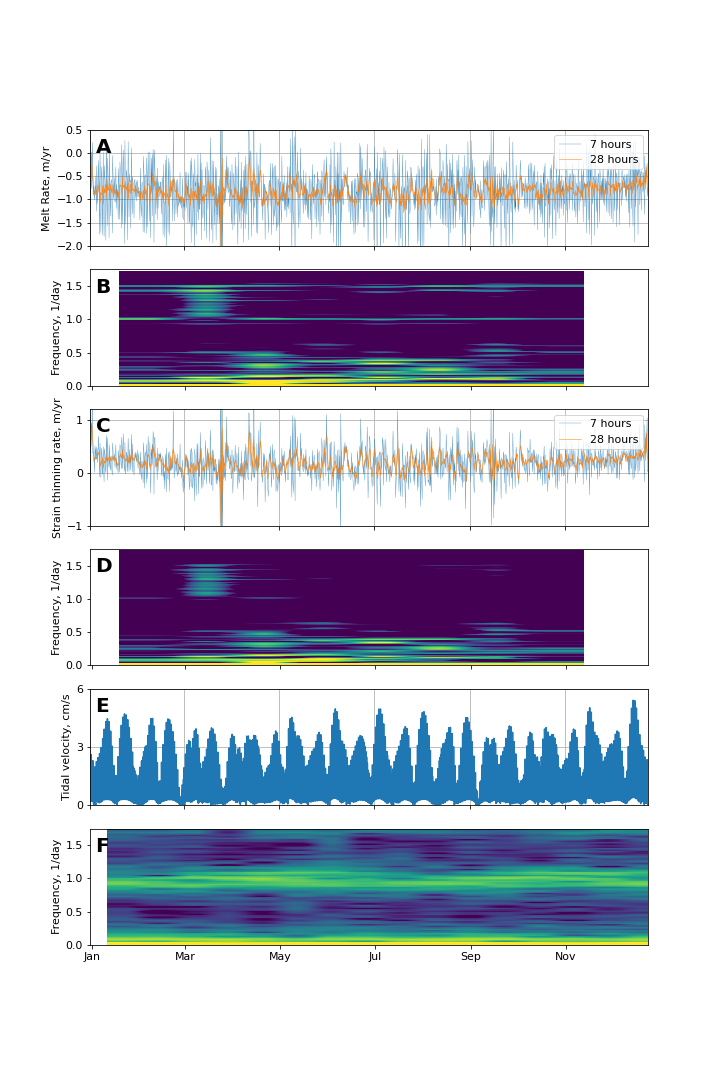
\includegraphics[width=0.7
\textwidth]{chapters/3/alltimeseries.png}
\caption[]{A) Time series of apparent accretion calculated at 7--hr intervals (blue line), overlaid by 28 hour intervals (orange line). Errors for the 28 hour interval time series are shown by shaded transparent orange areas. B) Spectrogram of the time series shown in (A), derived using the 28 hour rolling interval. C) Time series of strain thickening calculated at 7--hr intervals (blue line), overlaid by 28 hour intervals (orange line). Errors for the 28 hour interval time series are shown by shaded transparent orange areas. D)  Spectrogram of the strain thickening time series, derived using the 28 hour rolling interval. E) Time series of estimated tidal velocity magnitude at the channel using output provided by \cite{padman2002new}. F) Spectrogram of the tidal time series.
}
\label{fig:alltimeseries}
\end{figure}


\begin{figure}[!ht]
\centering
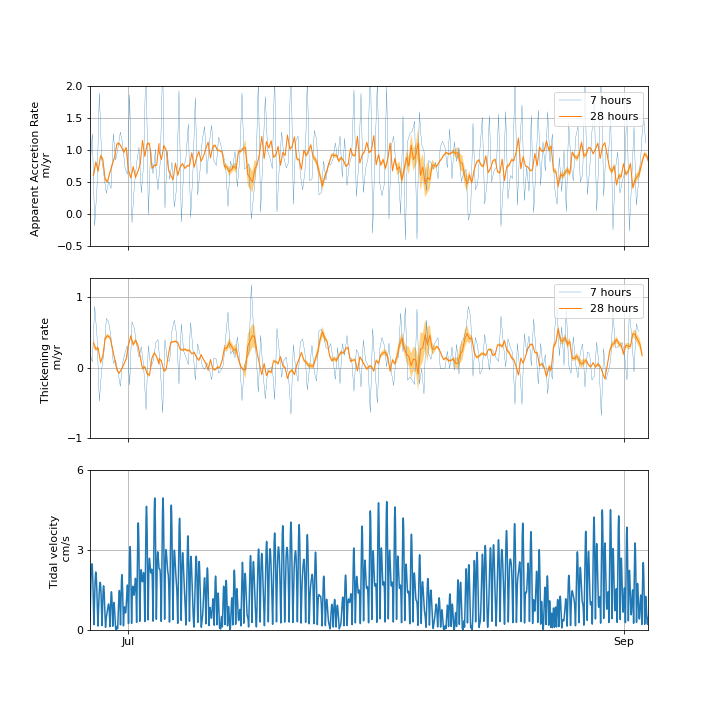
\includegraphics[width=0.7
\textwidth]{chapters/3/zoom_timeseries.png}
\caption[]{Data from time series as in Figure \ref{fig:alltimeseries} zoomed in on the month of July. A) Apparent accretion as in Figure \ref{fig:alltimeseries} A. B) Strain thinning as in Figure \ref{fig:alltimeseries} C. C) Time series of estimated tidal series as in Figure \ref{fig:alltimeseries} E.  
}
\label{fig:zoom_timeseries}
\end{figure}




\begin{figure}[!ht]
\centering
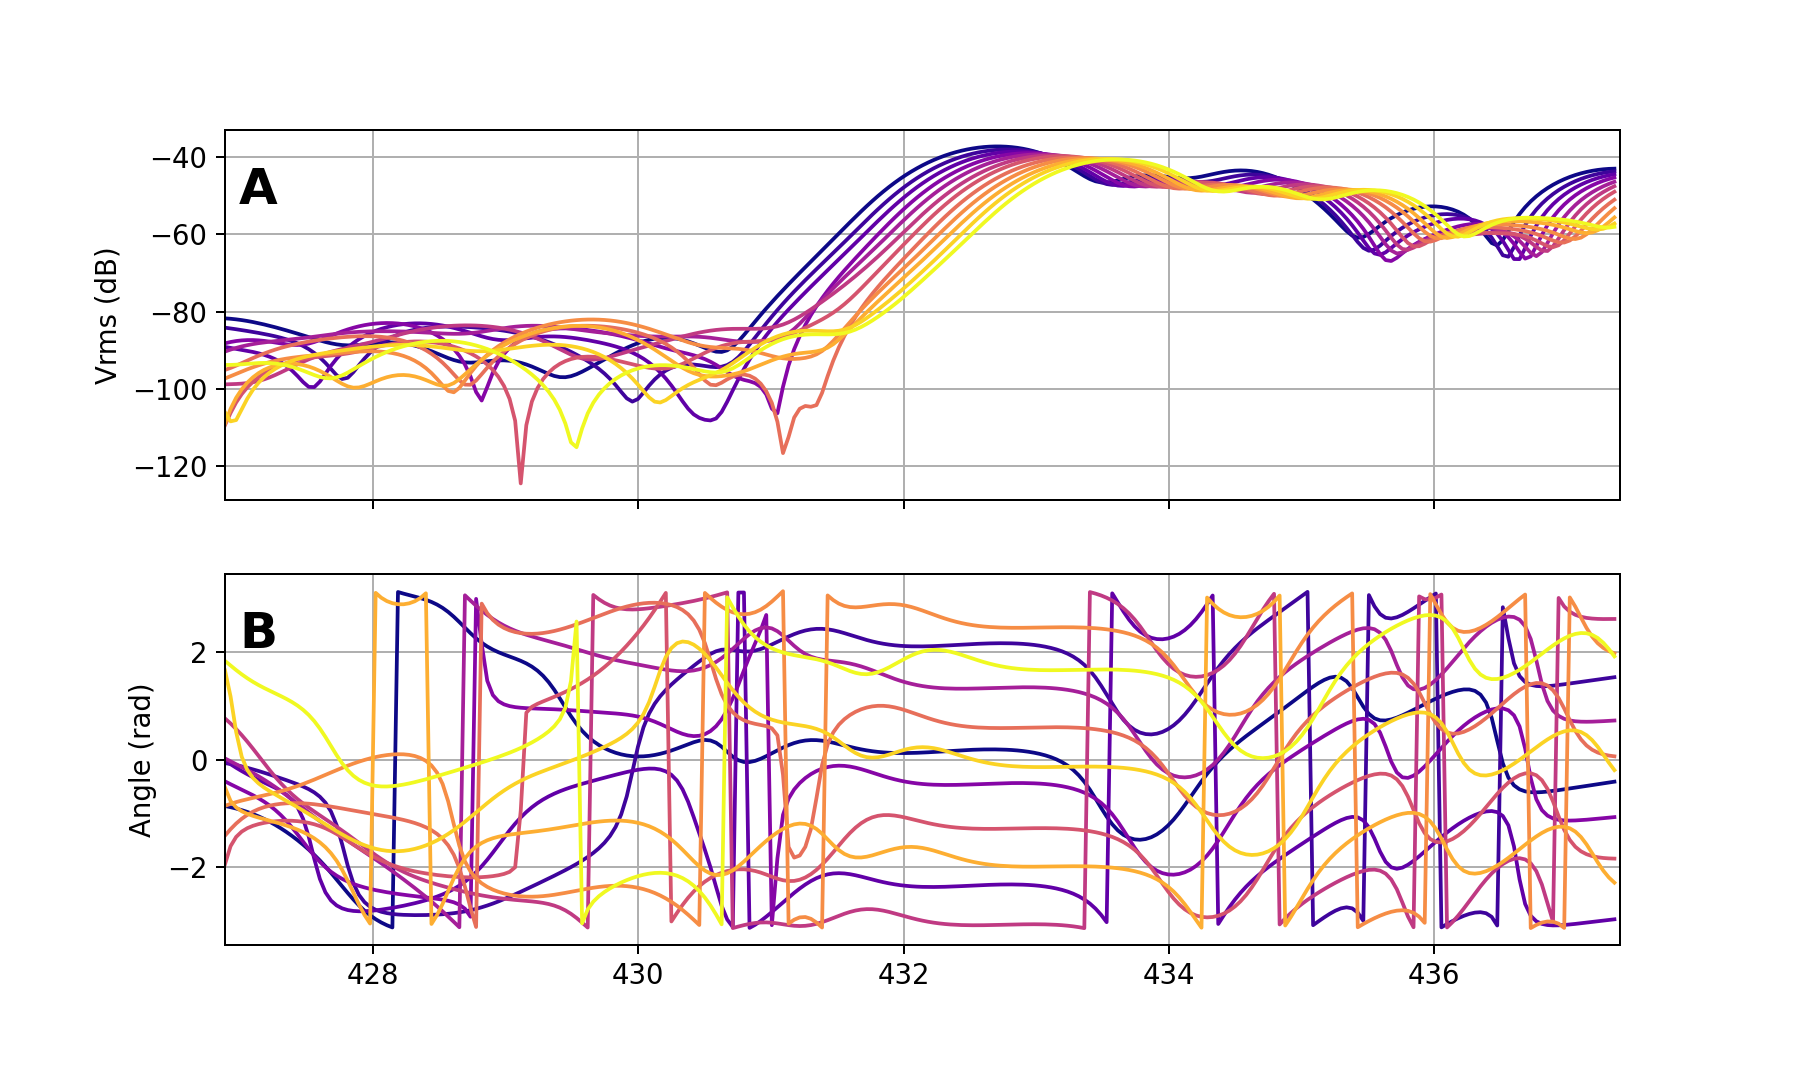
\includegraphics[width=0.7\textwidth]{chapters/3/range_amp_phase.png}
\caption[]{12 separate ApRES observations over 12 months of 2020. A) Range vs Amplitude, B) Range vs Phase. X--axis is zoomed in on the basal reflector at 433 m. Each line is calculated from the 1st of each month of 2020. Cool colours start in January, warm colours end in December. 
% C) Line of best fit through change in internal reflectors.
}
\label{fig:range_amp_phase}
\end{figure}

\newpage



% WHAT ABOUT CALCULATING STRAIN AT DIFFERENT INTERVALS

\begin{figure}[!ht]
\centering
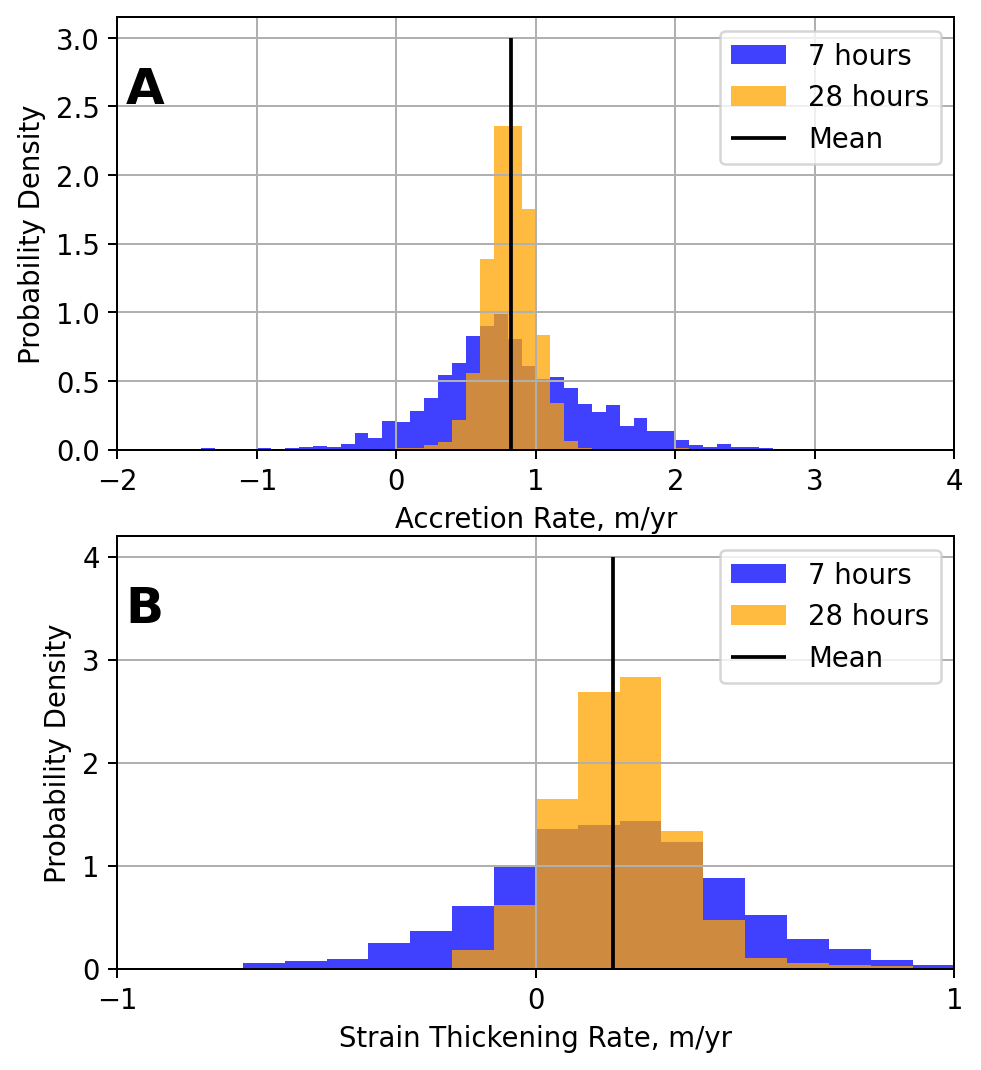
\includegraphics[width=0.5\textwidth]{chapters/3/histogram.png}
\caption[]{Histograms showing the variation in A) Accretion, B) Strain, over the time series. 
% C) Power Spectral Density of amplitude by Welch's average periodogram method.
}
\label{fig:histogram}
\end{figure}

Figure \ref{fig:alltimeseries} A shows a time series of apparent accretion from the 1  January 2020 to 23 December 2020.  Each data point is calculated from two ApRES observations made from $\pm$ 3 1/2 and $\pm$ 14 hours for the 7 and 28 hour sliding intervals respectively. Note that `apparent accretion' represents an increase in thickness and corresponds to the negative of `melt rate' as described in most ApRES research \cite[e.g.][]{vavnkova2021nature,lindback2019spatial}.
For both 7 and 28 hour intervals, apparent accretion fluctuates around an average of 0.81 m/yr  for the duration of the time series (Figure \ref{fig:histogram}), with median errors  of 0.07 and 0.03 m/yr respectively (Figure \ref{fig:alltimeseries} A).  The degree of variability is strongly dependent on the interval length, with longer intervals smoothing the apparent accretion in time (Figure \ref{fig:zoom_timeseries}). The 7 hour interval time series has lower and upper quartiles of 0.5 m/yr and  1.1 (Figure \ref{fig:histogram}), and the 28 hour interval time series has quartiles of 0.7 and 0.9 m/yr (Figure \ref{fig:histogram}) . The spectrogram of apparent accretion (Figure \ref{fig:alltimeseries} C), which is calculated with 28 hour intervals, shows dominant short periods of 16, 18 and 24 hours and a weakly dominant period of 26 hours. Longer 14 day periods are strongly dominant from January until around October, and 2 and 4 day periods are intermittently dominant. 

Strain thinning rate varies in amplitude throughout the time series around a mean of 0.2 m/yr (Figure \ref{fig:histogram}) with a mean strain rate error of 0.03 m/yr. Strain calculated over 28 hour intervals have lower and upper quartiles of 0.12 and 0.27 m/yr  respectively (Figure \ref{fig:histogram}).   With a mean ice thickness of 433 m, this corresponds to a strain rate of 4.6 x $10^{-4}$ / yr
Strain is generally positive, showing longitudinal compression or thickening due to strain in the area (Figure \ref{fig:example_signal} and \ref{fig:12strains}). On average, strain contributes to  24\% of the apparent accretion. The periodigram of strain (Figure \ref{fig:alltimeseries} C) shows 14 days periods are strongly dominant from February until around October. %quantify strongly
Periods of 1, 2 and 4 days are intermittently dominant.

\begin{figure}[!ht]
\centering
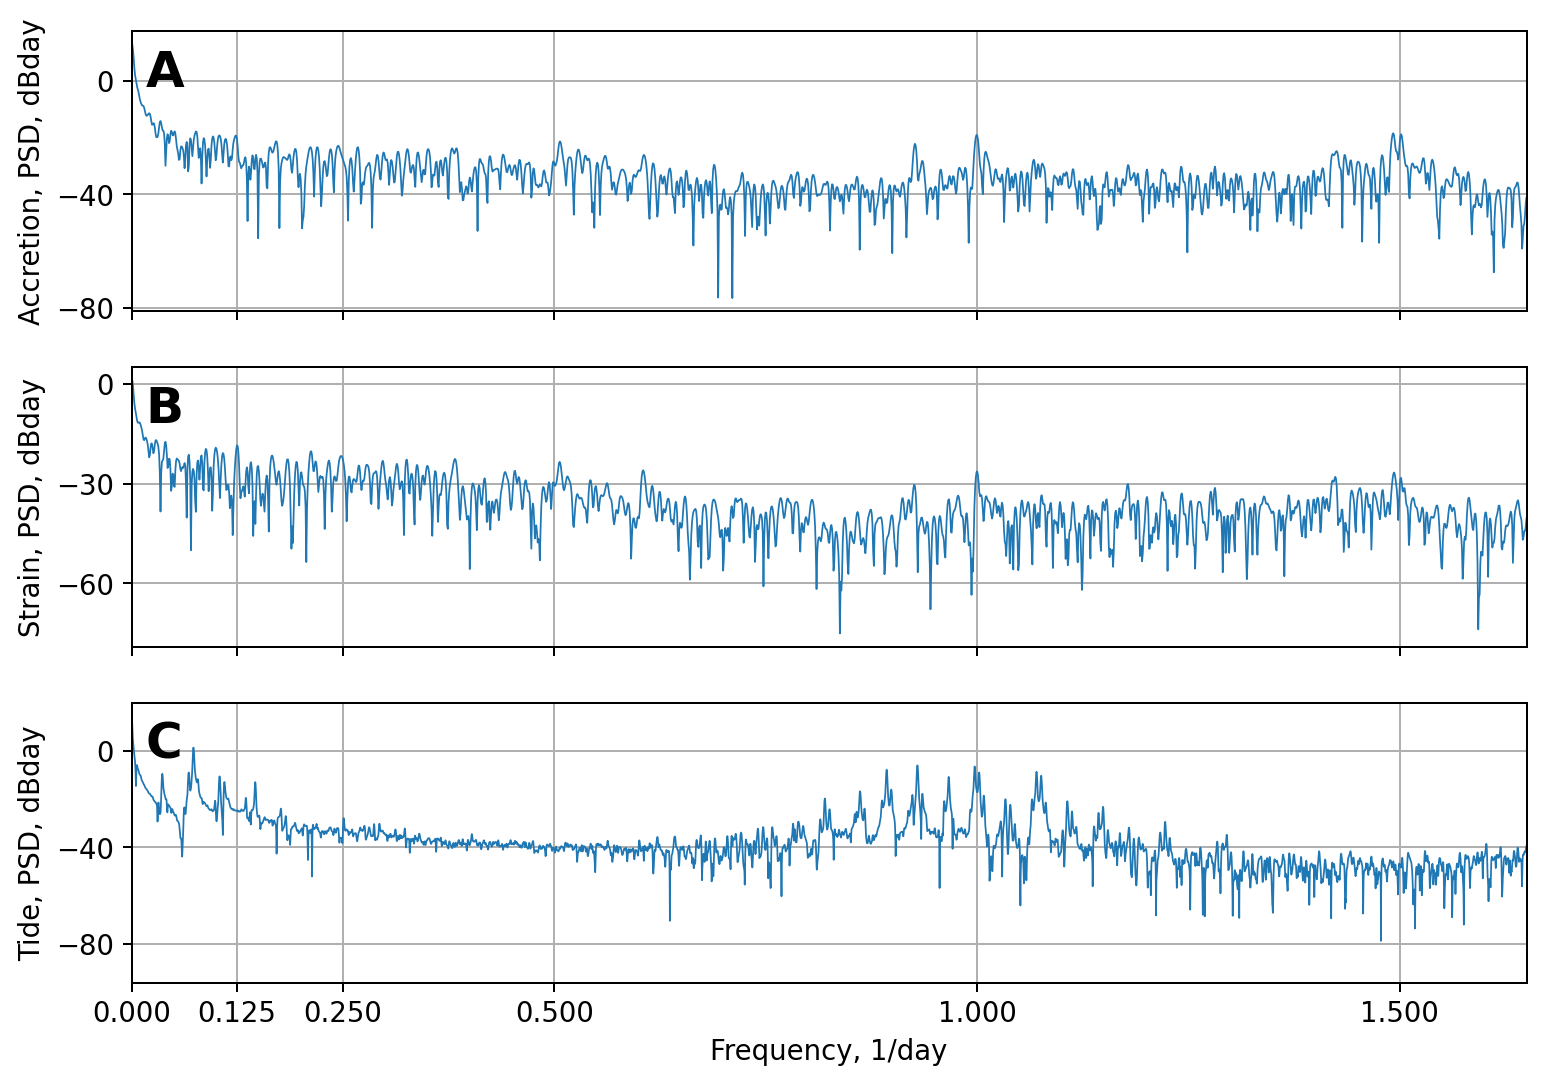
\includegraphics[width=0.7\textwidth]{chapters/3/spectral_density.png}
\caption[]{The Power Spectral Density (PSD) of  apparent accretion (A), strain (B), and estimated tidal magnitude (C) from \cite{padman2002new}. Power Spectral Density is calculated by Welch's average periodogram method. A and B are calculated from time series calculated over 28 hour intervals.
}
\label{fig:spectral_density}
\end{figure}

The power spectral density (Figure \ref{fig:spectral_density}) of apparent accretion calculated at 28 hour intervals over the entire time series shows diurnal and semidiurnal periodicity with local maximums at frequencies of 0.5, 0.93, 1, 1.42 and 1.5 per day. These correspond to periods of 48, 26, 24, 17 and 16 hours respectively. The power spectrum of strain thickening also has local peaks at these frequencies, and additionally, has local peaks at 0.6 and 1.2 per day which correspond to periods of 20 and 40 hours respectively. 
% For both strain and apparent accretion, power spectral density is $\approx 10$ dBday higher for low frequencies (less than $\approx$ 0.5 per day), with no clearly dominant frequencies.


\subsection{Sliding interval method}

\label{sec:synthetic}
\begin{figure}[!ht]
\centering
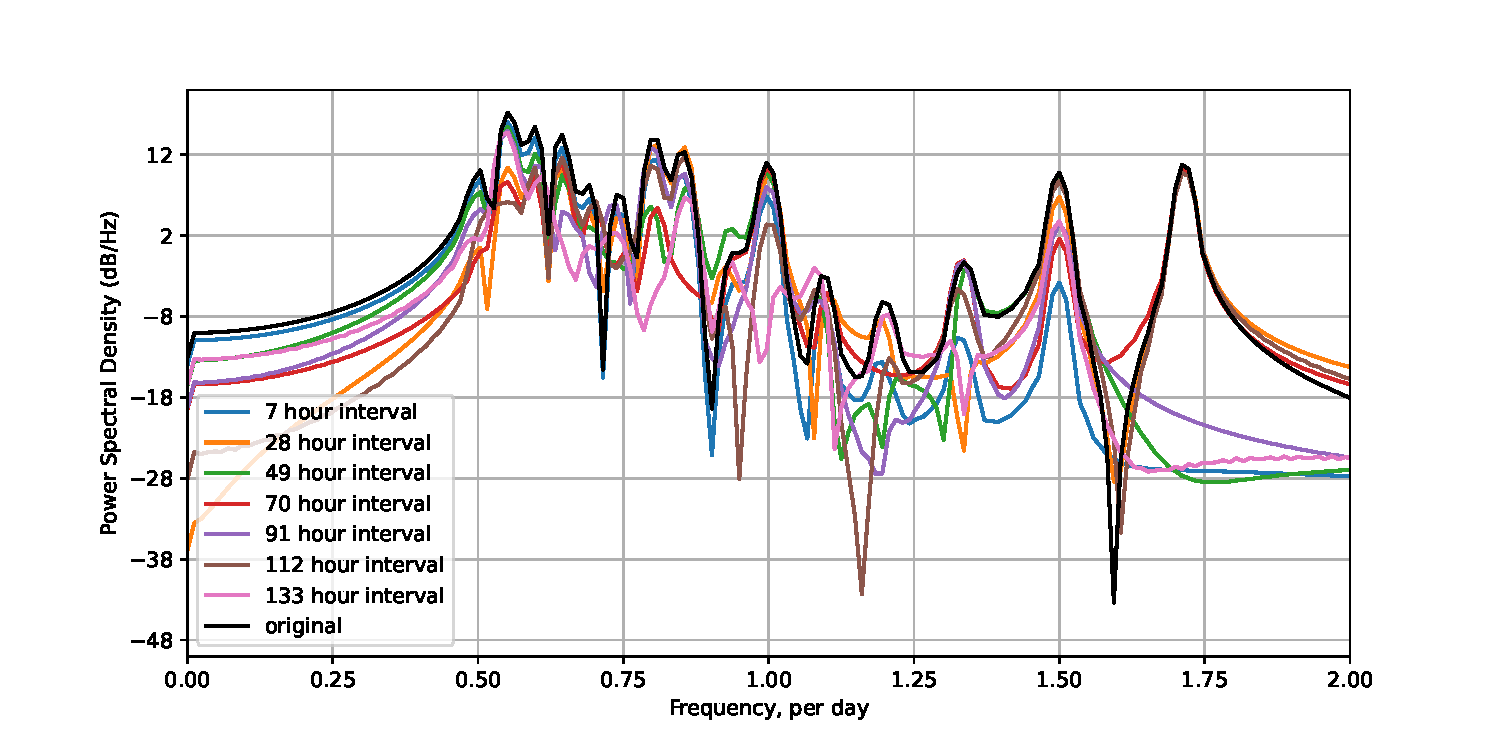
\includegraphics[width=1\textwidth]{chapters/3/synthetic.pdf}
\caption[]{In black, the power spectrum of a synthetic time series which is the addition of randomly sine waves with periods from 14 to 50 hours. Colours show power spectrum of the time series resampled over different intervals as $y[n] = (x[n-w/2]+x[n+w/2])/2$ where $x$ is the original time series, $y$ is the resampled time series and $w$ is the interval length.}
\label{fig:synthetic}
\end{figure}

Calculating strain and melt over larger intervals has the effect of smoothing the apparent accretion (Figure \ref{fig:alltimeseries}). The effect of a large interval on frequencies is that similar to a comb filter. The output of the filter periodically drops to a local minimum at multiples of the interval frequency $1 / 2T_w, 3 / 2T_w, 5 / 2T_w \cdot$, where $T_w$ is the interval width. The distortion to frequencies is therefore specific and different for each interval length. Figure \ref{fig:synthetic} shows the effect of interval size on a synthetic time series. The time series is a random sum of sine waves with periods from 14 to 50 hours, which we resample using a sliding average of two points to simulate our melt rate calculations. The sliding average is defined as $y[n] = (x[n-w/2]+x[n+w/2])/2$ where $x$ is the original time series, $y$ is the resampled time series and $w$ is the interval length. The resampled time series show similar patterns of frequency distributions though the amplitudes of certain frequencies change. Longer intervals show the most distortion, filtering out frequencies greater than 1.5 1/day, and showing less fidelity than shorter intervals for frequencies greater than 1.5 1/day. Intervals of 7 and 28 hour demonstrate good fidelity.

\begin{figure}[!ht]
\centering
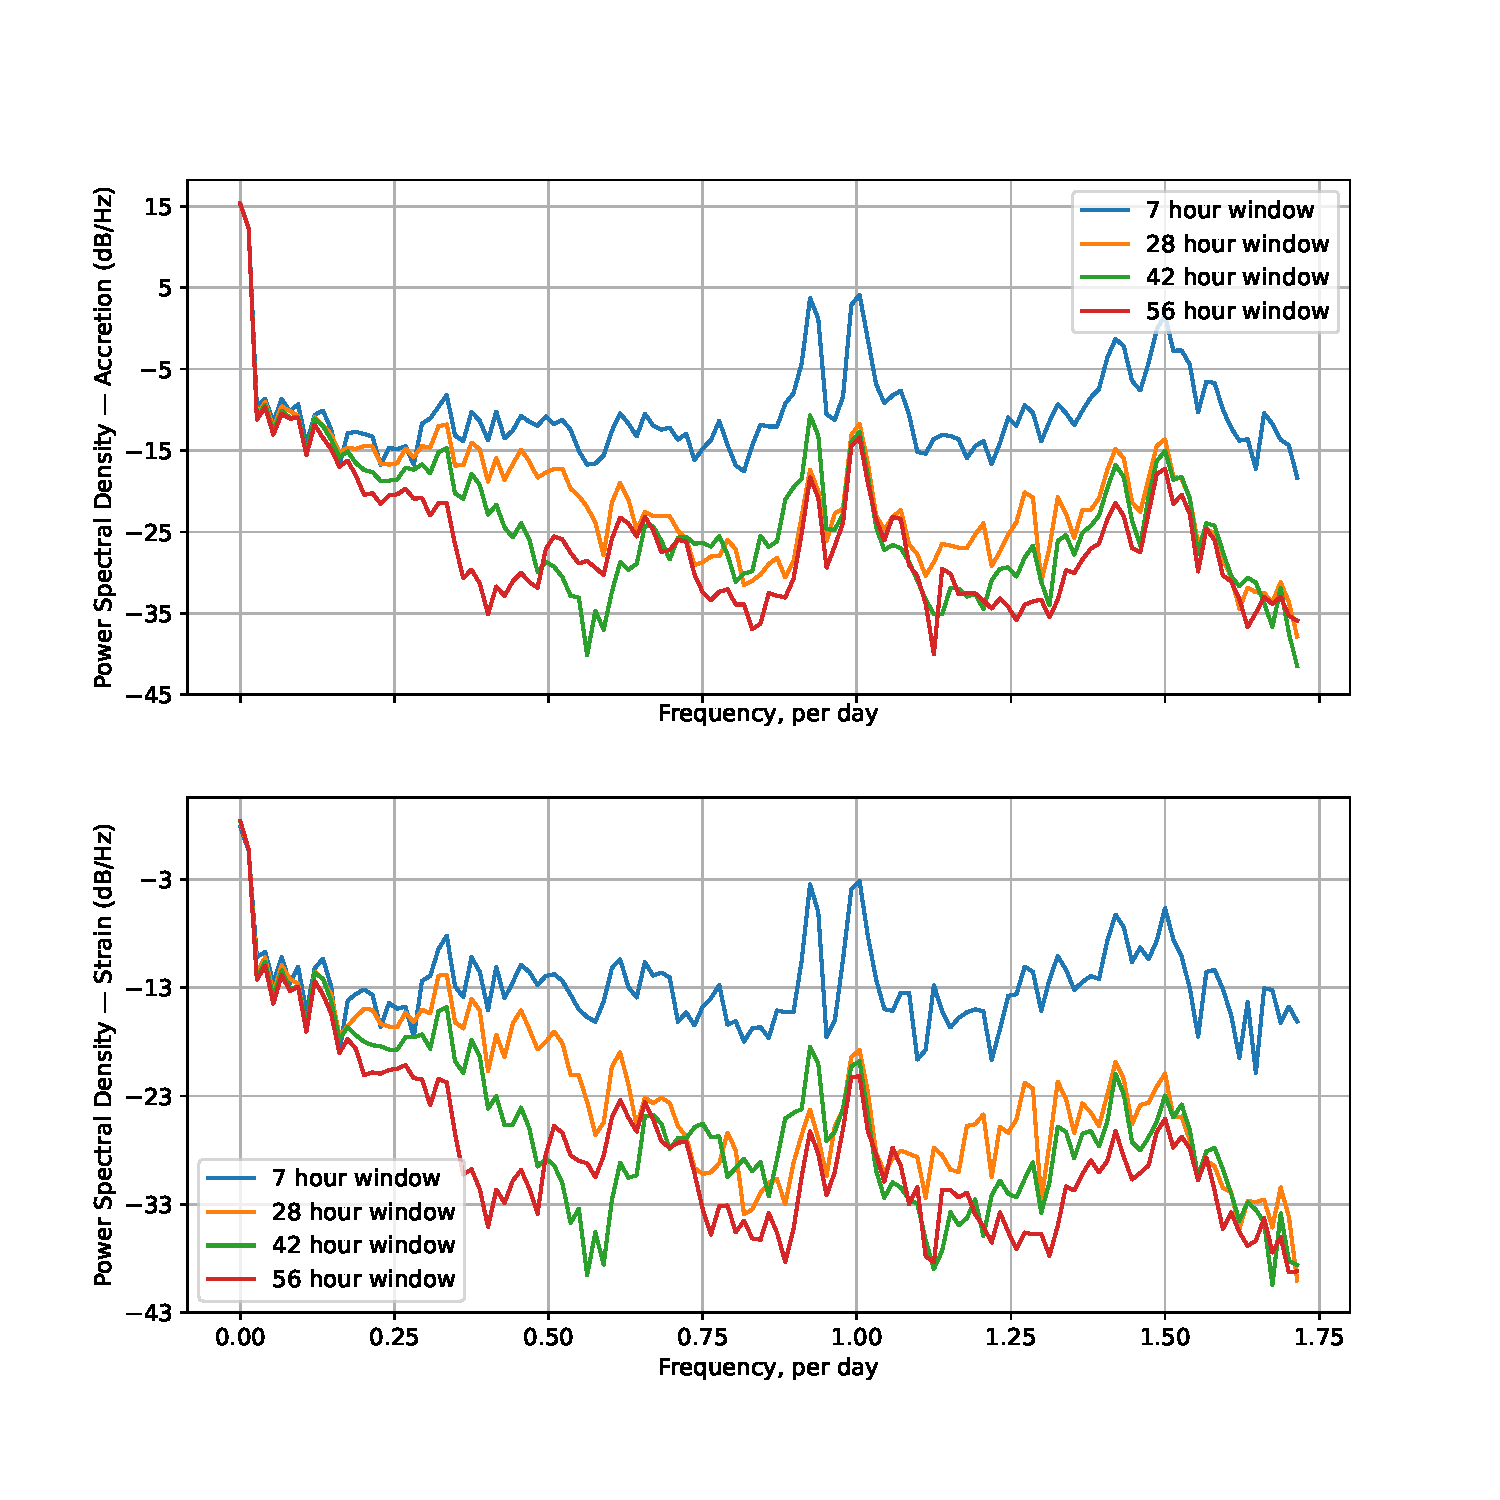
\includegraphics[width=1\textwidth]{chapters/3/compare_window.pdf}
\caption[]{Power spectrum of ApRES time series for apparent accretion (top) and strain (bottom) for a range of different sampling intervals, shown by different colours.}
\label{fig:compare_window}
\end{figure}
We compare the power spectrums (Figure \ref{fig:compare_window}) of the ApRES melt and strain thickening time series with a range of interval sizes. Figure \ref{fig:compare_window}  shows which frequencies are consistently dominant over different length intervals. In particular, a diurnal signal is dominant regardless of the interval size. This shows that the increase in uncertainties in strain caused by smaller (7 and 28 hour) intervals does not introduce artefacts in the power spectrum which have caused these frequencies to be dominant. This justifies the sliding interval method of calculating melt rates, described next.


% plots 
\subsection{Amplitudes}

\begin{figure}[!ht]
\centering
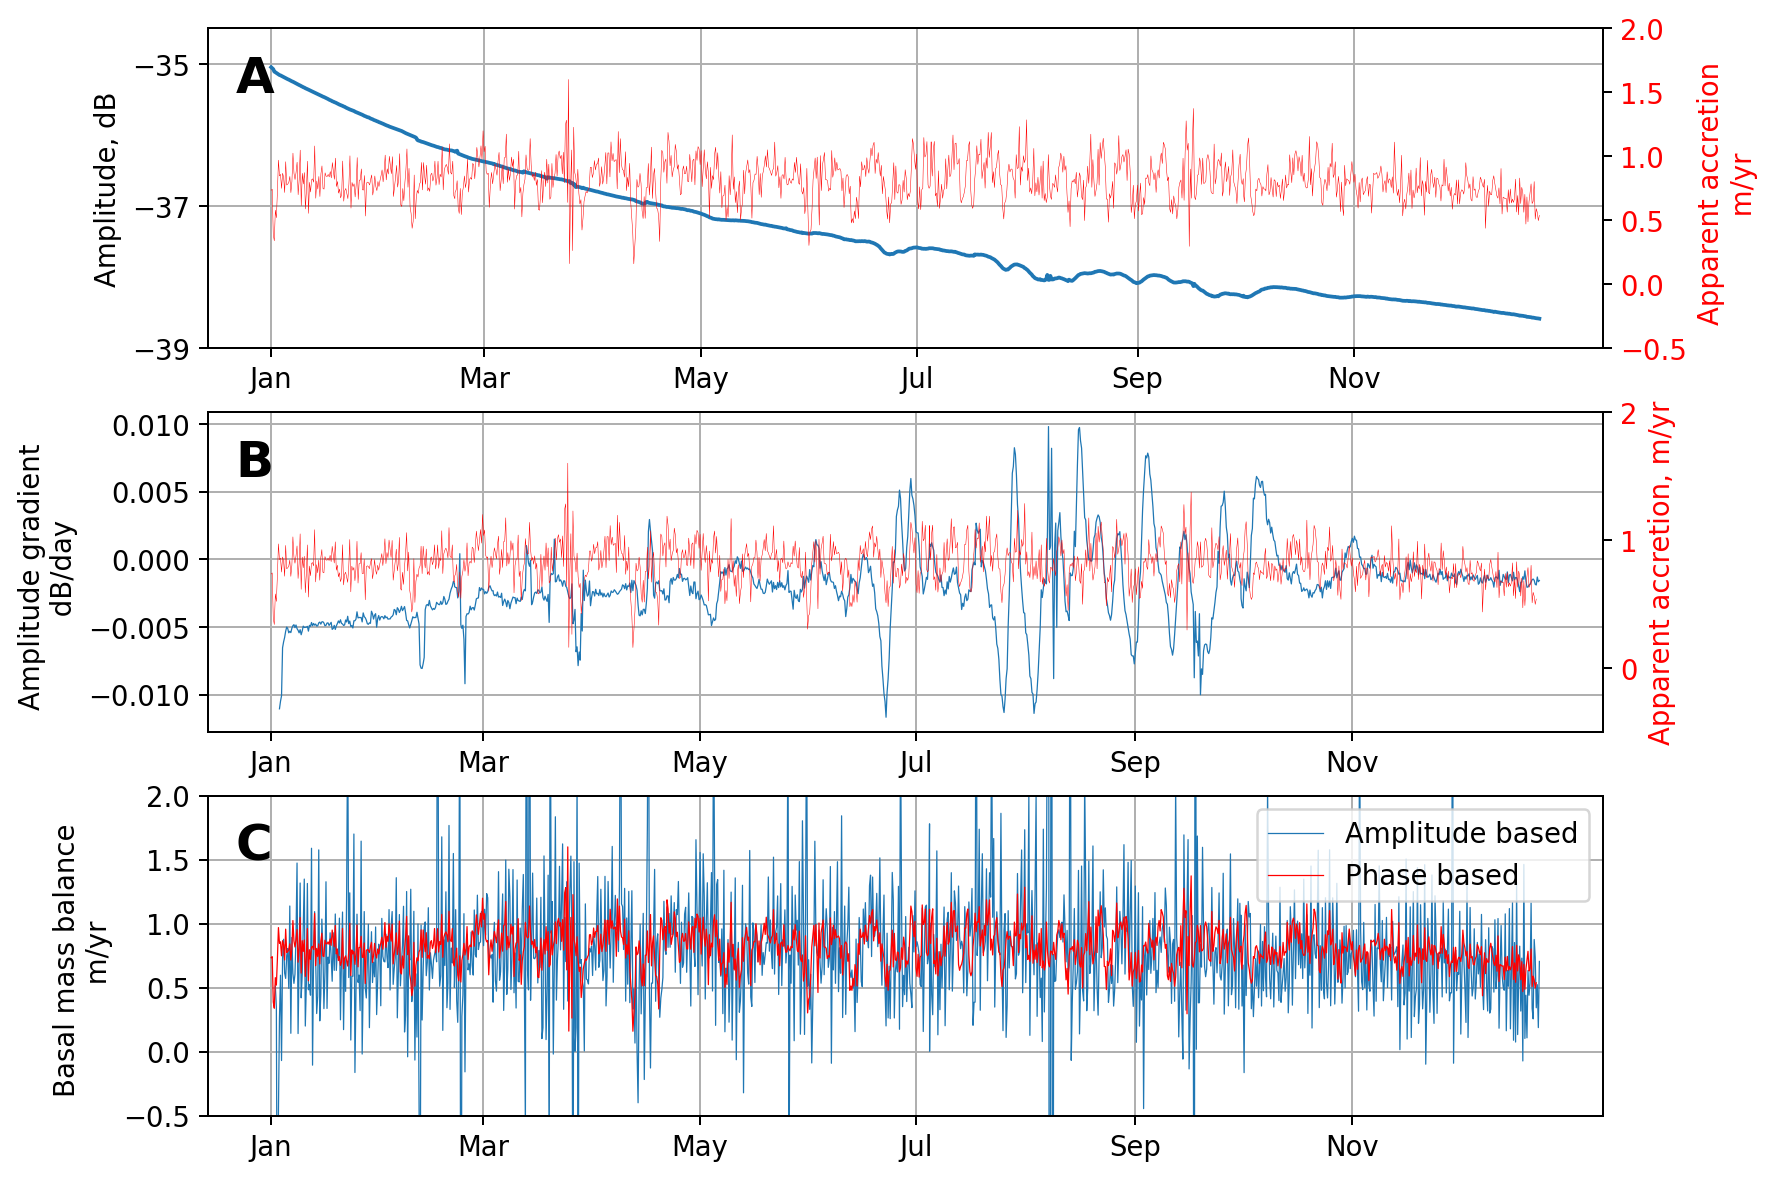
\includegraphics[width=1\textwidth]{chapters/3/amplitudes.png}
\caption[]{A) Time series of amplitudes of basal reflector in blue overlay estimated apparent accretion in red. B) Amplitude and apparent accretion shown from March and April to show more detail. C) `Apparent accretion' is the basal mass balance calculated from phase. Here compared to the basal mass balace calculated by tracking amplitude.
% C) Power Spectral Density of amplitude by Welch's average periodogram method.
}
\label{fig:amplitudes}
\end{figure}
% period
A time series of return amplitude over 2020 shows a negative trend in the amplitude of the basal reflector, from -35.0 dB to -38.6 dB. 
The gradient is steepest in January, and sees the most variability from April to October. No spikes in amplitude exceed 2 dB.
The basal mass balance calculated from tracking the amplitude of the basal reflector matches the apparent accretion, which is the basal mass balance calculated from phase. The changing range to the amplitude of the basal reflector is shown in 
Figure \ref{fig:range_amp_phase}. The amplitude based  basal mass balance displays significantly more noise than the phase derived basal mass balance. The mean of the amplitude based  basal mass balance is 0.78 m/yr, slightly less than the mean of apparent accretion which is 0.81 m/a.

\newpage

\section{Discussion} \label{sec:apres_discussion}

\subsubsection{What does the observed apparent accretion represent?}

%%%%%%%%%%%%%%%%%%%%%%%%%%%%%%%%%%%%%%%%%%%%%%%%%%%%%%%%%%%%
% primary conclusion is that there is marine ice.

%there is marine ice shown by no melt
We suggest that for the duration of the time series presented (Figure \ref{fig:alltimeseries}), the base of the ice shelf below the ApRES instrument consists of a layer of marine ice, which has accreted to the bottom of glacial ice. Evidence for a basal marine ice layer comes from ApRES observations of consistent apparent accretion throughout the time series (Figure \ref{fig:alltimeseries} A). Consistent apparent accretion rules out the possibility that the base is purely glacial ice, which can only exist under active melting or zero mass balance.
% Similarly, other studies have found marine ice layers under the Ross Ice Shelf \cite[e.g.][]{das2020multidecadal,macgregor2011grounding}. 
% marine ice existence confirmed by amplitude
In addition, the amplitude of apparent accretion (Figure \ref{fig:amplitudes}) shows a smooth change throughout the time series, gradients do not exceed 0.01 dB/day, implying no sharp change in the properties of the dominant reflector  \citep{vavnkova2021nature}. This confirms that basal conditions are consistent throughout the time series, confirming the existence of basal ice. Previous work by \cite{vavnkova2021nature} suggests that the temporal change from a base of glacial ice to a base of marine ice, or vice versa, causes a sharp change in the amplitude ($\gtrapprox$0.25 dB/day) of an ApRES reflection. 

%%%%%%%%%%%%%%%%%%%%%%%%%%%%%%%%%%%%%%%%%%%%%%%%%%%%%%%%%%%%
% next conclusion is that this marine ice is changing. and that its consistent confirmed by consistent amplitude and no jumps
The apparent accretion displayed throughout the time series (Figure \ref{fig:alltimeseries} A), shows a consistently changing dominant reflection from the ice base. This is most likely caused by a consistent change in the marine ice layer. 
Assuming there is a layer of marine ice present at the base of the ice shelf, we expect the ApRES to return a strong reflection from the glacial/marine--ice boundary due to the strong dielectric contrast and possibly a second, weaker reflection from the marine--ice/sea boundary (as in \cite{fricker2001distribution}).
Apparent accretion shows that the apparent range, the distance from the ApRES instrument to the main reflector, is increasing (Figure \ref{fig:alltimeseries}). This is likely caused by a change in the interference of reflections from the glacial/marine--ice interface and the marine--ice/sea interface. The addition of reflections is likely causing a phase shift which appears as an increase in the range to the resulting reflection \citep{vavnkova2021nature}. It is unlikely that the increase in apparent length is caused directly by an increase in length caused by accretion, because it is unlikely that the main reflection is at the marine--ice/sea boundary, which has a weaker dielectric contrast than the glacial/marine--ice boundary.
The change in interference of the two reflections could be caused by accretion, or melt, and/or a change in the electromagnetic properties of the marine ice. Depending on the thickness and properties of the marine ice, accretion or melt could result in an increase in the apparent length \citep{vavnkova2021nature}.

Following the work of \cite{vavnkova2021nature}, due to the unknown potentially changing properties of the accreted marine ice layer, we cannot be certain as to whether the basal interface is melting or accreting. 
% vavnkova says we cant tell whats happening at the base
\cite{vavnkova2021nature} modelled relationships between the change in thickness of the accreted layer and change in phase shift and basal amplitude.  They found that for an observed change in apparent length, there are a number of different possible solutions. The apparent length is a function of the thickness, the dielectric constant, and the electrical conductivity of the marine ice layer. The relationships between these variables and apparent thickness also depend on the frequency of the radar signal. \cite{vavnkova2021nature} found that it is not always possible to constrain apparent accretion rates without a better understanding of the thickness and properties of the marine ice layer.

% The consistently positive apparent accretion likely represents a consistently positive or negative change in basal mass balance. Consistently negative mass balance would eventually melt through the marine ice to glacial ice, which we do not see. 

We suggest there are three potential explanations for the observed apparent accretion (Figure \ref{fig:alltimeseries}). 
The most likely is the simplest explanation that ice is actively accreting throughout the time series. The consistent apparent accretion is probably caused by consistent accretion as in \cite{vavnkova2021nature}, where the accuracy of switches between apparent accretion and melt were confirmed by the growing and disappearing of a marine ice layer. Both phase and amplitude based apparent accretion (Figure \ref{fig:amplitudes} C) show a consistent positive basal mass balance throughout the time series, suggesting that phase changes are caused by a change in the range, and not by changes in the dielectric contrast of the boundaries. This supports the explanation that the observed apparent accretion is caused by basal accretion.

Secondly, it is possible that the ApRES site had thick marine ice  before the time series, and during the time series the layer is actively melting resulting in signals which appear as apparent accretion. This would require the peak and phase to be distorted by destructive interference from multiple reflections. If one of the reflections had a shift in polarity, then a decrease in range (caused by melt) to the marine ice base could combine with the stable reflection from the glacial/marine ice boundary to show an increase in the range of the dominant reflector (showing apparent accretion).
This would imply that the base has gone through different periods of accretion and melt, and that the time series caught a snapshot of just the melt period. Consistently negative mass balance would eventually melt through the marine ice to glacial ice, which we do not see.  If outflow through the channel is episodic, large floods of subglacial water passing through (as suggested in Chapter \ref{ch:data}) could cause the accumulation of thick marine ice on the bottom of the ice shelf. It is possible that for the year of 2020 this marine ice was consistently melting. 

Thirdly, is is feasible that basal ice is metamorphosing in a way which steadily changes its electromagnetic properties through the time series. If true, basal ice metamorphosing must be influenced by tidal forces, as we can see tidal signals in the apparent accretion. This scenario is unlikely, as it is unlikely that changing electromagnetic properties of the basal layer would result in consistent basal mass balance estimates from both phase and range (Figure \ref{fig:amplitudes}).  This possibility is difficult to support or rule out, as we know little about the changing electromagnetic properties of metamorphosing marine ice. 

% There is very little knowledge of the relationships between  metamorphosing marine ice and  is can cause the electromagnetic properties to change.

%IDEAS FOR WHY ONE MOST LIKELY
% There is no in--situ evidence of basal ice metamor The only evidence we have of basal ice metamorphosing suggests that this happens consistently, and not with oscillations which we observe with tidally related oscillations, it follows  that we cannot asuggest that this is the least likely explanation for the observed accretion.

% huw.horgan: Separate each of these possibilities out. Substantiate them with whatever evidence you may have presented in your results. Discuss which you think is most likely and why. Then discuss the implications of this.

% However, it is most likely that the apparent length increase is being caused by accretion or melt on a basal marine ice layer: 
% Firstly, we can observe apparent accretion over small time scales. It is unlikely that changes in the electromagnetic properties of the marine ice occur fast enough to cause these. Secondly, we see the same trend of increasing apparent length thoughout the time series, and the same trend of shrinking amplitude throughout the series.  \cite{vavnkova2021nature} finds that at the onset of accretion, amplitude sharply decreases. Amplitude doesnt decrease until the accreted ice is melted away. 
% % The change in apparent length is likely caused by a change in the interference of reflections from the glacial--marine ice interface.
% The apparent accretion shown for the duration of the time series (Figure \ref{fig:alltimeseries} A) likely shows a change in the reflection from the glacial/marine--ice boundary.



\subsection{Drivers of mass balance variability}

The apparent accretion time series shows diurnal periodicity (Figure \ref{fig:alltimeseries} A) which we attribute to the tidal influence on circulation and melt in the channel. 
Specifically, periods of 26 and 24 hours are dominant in both the apparent accretion time series (Figure \ref{fig:spectral_density} A) and the estimated tidal velocity time series (Figure \ref{fig:spectral_density} C).
50km from the ApRES location at `KIS1' ( Figure \ref{fig:ris}), \cite{robinson2020ice} estimated a basal melt rate time series from oceanographic observations, and found that basal melt rates closely followed diurnal tides. 
Additionally, internal tidal waves between layers in the cavity like those described by \cite{robinson2020ice} likely promote mixing.  Because the channel is constricted, the tide is expected to behave differently from the larger Ross Ice Shelf cavity. The shape of the channel is similar to a converging (upstream narrowing) esturine river mouth, which generally enhance tidal amplitude \citep{van2011analytical}.

\cite{lindback2019spatial} similarly found diurnal basal melt fluctuations using ApRES on the Nivlisen Ice Shelf, and attributed these to tide--driven circulation.
\cite{makinson2011influence} modelled circulation under the Filchner-Ronne Ice Shelf, and showed that tides increase basal melt by enhancing cavity circulation, increasing both the outflow of cold water and inflow of warm saline water. They found that the presence of tides doubled estimated basal melting under the Filchner-Ronne Ice Shelf. While both of these examples show melt not in a basal channel, melt in basal channels is thought to occur from similar processes to outside, through meltwater plumes \citep{sergienko2013basal} and the circulation and recycling of melt water with warmer saltier water.
 
%  Relative to other ApRES sites, the time series does not show strong variability.  For example, \cite{vavnkova2021nature} observed basal mass balance fluctuating between melt and accretion, or \cite{davis2018variability} who observed melt rates fluctuate from 0 to 8 m/a. Even with strong variability, \cite{davis2018variability} has difficulty explaining what caused the variability.
% Changes in basal mass balance at the scale we observe could happen from something as simple and variable as the change in the flow in an eddy. 
 
  
\subsection{Strain thinning} 
 
Observations of consistent positive strain thickening over the ice column (Figure \ref{fig:alltimeseries} D) suggest a viscous response to localised basal melt.  While our observations at the ApRES location reveal basal marine ice, and potential thickening, the channel shape shown in Figure \ref{fig:4square_channel} shows the location previously saw more than 300 m of ice  melt. Ice is likely flowing towards the centre of the channel to compensate for the melt driven formation of the channel.
In theory, this strain thickening will not cause crevassing like that observed by strain thinning \citep[e.g.][]{vaughan2012subglacial}. If anything, the strain thickening will cause the closing of crevasses.
We discount significant active flexing as a cause of strain, as the effect of flexure on strain would be thickening in the upper half of the ice column and  thinning in the lower half \citep{vaughan2012subglacial}, which is not observed (Figure \ref{fig:example_signal} shows strain thickening throughout the entire ice column).
In comparison to 4.6 x $10^{-4}$ / yr at our site \cite{alley2018continent} finds that the along flow strain rate in the area is positive and $< 1 \times 10 ^{-6}$/a, and the transverse strain rate is close to zero, $< 1 \times 10 ^{-6}$/a.

Apparent accretion is the sum of strain thickening rate and the rate of change in range to the basal reflector. While strain thickening contributes to just 24\% of the apparent accretion estimates over the whole time series, variation in apparent accretion is closely related to strain thickening. This is clearly evident when comparing zoomed in apparent accretion and strain thickening in Figure \ref{fig:alltimeseries} B and E, and is also shown by the similar spectrograms of Figure \ref{fig:spectral_density} A and B. While this close correlation could be caused by errors in the melt rate calculation method, there is no clear evidence of such errors. Calculated strain thickening rate errors are small relative to the signal. These errors are calculated by the quality of fit as shown in Figure \ref{fig:12strains}, which confirms we have a linear strain profile, and the linear fit is reasonable. 
Using larger intervals (up to 100 hours) to calculate strain thickening rates results in similar close correlation of oscillations between strain thickening and melt rate, with similar dominant frequencies (Figure \ref{fig:compare_window}). This suggests that the length of our interval is robust, and is not corrupting strain thickening rate calculations. 
The close correlation of strain thickening and melt rates is most likely due to the fact both melt and strain thickening are principally driven by the same external forces. In this case, external forces such as tides drive apparent accretion and strain thickening to vary in sync. Alternatively, the correlation could be due to the dependance of melt rate on strain thickening rates or vice versa.  For example, it is possible that feedbacks stabilise the basal elevation,  resulting in a basal mass balance which essentially cancels out the strain thickening. This is an unlikely explanation, as melt and accretion feed backs caused by changes in the strain, or the converse, are unlikely to occur at the same time scales. 
% For example, with a vertically stratified, stable ocean column in the channel cavity, a lowering of the ice base due to strain thickening would bring the ice interface into saltier waters, increasing melt. Conversely, a rise in the ice base would decrease salinity at the ice base, lowering melt rates. 
% Alternatively, an increase in basal melt would cause subaerial surface lowering which would induce strain thickening due to the increase in gradients in the subaerial ice surface slope.

\subsection{Implications of results on subglacial plume dynamics}
The existence of a layer of basal marine ice implies that the ApRES location has experienced positive basal mass balance in the past. Either supercooled water accretes directly to the ice at the site, or frazil ice carried by currents accumulates and builds a layer of marine ice \citep{vavnkova2021nature}.  Accretion is likely driven by a meltwater plume as described by \cite{hewitt2020subglacial}. Subglacial discharge initiates a meltwater plume which flows up the face of the ice, melting ice, becoming fresher and more buoyant. The upward plume entrains warm salty water from the ocean depths to the ice face, enhancing melt. Plume theory (as in \cite{jenkins2011convection}) predicts melt for a certain distance downstream from the start of the plume, after which the the plume is predicted to lose energy and cause accretion. Our dataset provides constraints on the length scales over which a melt water plume loses energy, in that accretion can occur 3 km downstream from the inception of the channel.

The formation of marine ice immediately downstream from the melt region adds constraints to our conceptual model of the channel formation discussed in Chapter Data (where we suggested that the channel had formed through the upstream step--wise migration of a subglacial plume). The ApRES location spot was likely a focus of basal melt at some time in the past, when the surface basin formed, but now is downstream of the active melting part of the channel and is thickening. This implies that melt is relatively focused at the tip of the channel, which suggests that it has been throughout the channel formation. This reinforces the theory that a retreating subglacial plume has formed the channel, because localised melt must move in order to form a linear feature like the channel.

Additionally, we have theorised that for the duration of the year long time series there is a consistent basal mass balance. If we assume that accretion rates are influenced by a subglacial plume triggered by subglacial drainage, it follows that there are no major changes in subglacial drainage for the time period surveyed. 
We would expect changes in subglacial drainage to be associated with changes in basal mass balance at the ApRES location. 
Research by \cite{kim2016active} found that when lakes on the Kamb Ice Stream flood, variability is at sub--annual timescales.  It follows that the time series we present does not show the channel in a subglacial flood period. This implies that the channel is quiescent for over a year, and constrains a potential period of invariability in the channel.
If the observed accretion is driven by the melt water plume, we can also deduce that the melt water plume at the inception of the channel experiences tidal variability. This suggests that the plume has strong connections to the ocean.


\section{Conclusion}

We have presented a time series of Autonomous Phase-sensitive Radio-Echo Sounder (ApRES) observations taken at the apex of a sub ice shelf channel at the grounding line of the Kamb Ice Stream. The time series spans most of 2020, and shows basal marine ice for the entirety of the period. This is confirmed with analysis of the amplitudes of the basal reflection, which show no sharp changes through the time series. We interpret the consistent apparent accretion observed by the ApRES as a consistent basal mass balance with a marine ice layer underlying glacial ice.  We are unable to confidently constrain the mass balance as melt or accretion due to the unknown, potentially changing properties of the marine ice layer, though suggest that mass balance is most likely positive.  Mass balance has a strong diurnal signal, which we attribute to tidally--driven circulation. The estimated strain is consistently thickening in the area, which corresponds to a viscous response to the previous incision of the basal channel.


